%----------------------------------------------------------------------
% Antecedentes y estado del arte
%----------------------------------------------------------------------

\section{Antecedentes y estado del arte}
\label{sec:estado-arte}

\subsection{Evolución de los medios de pago hacia SEPA}
\label{subsec:evolucion-sepa}


El ecosistema europeo de pagos ha experimentado una profunda transformación en las últimas décadas, pasando de sistemas nacionales heterogéneos a un marco unificado bajo la iniciativa \textbf{SEPA}. Antes de SEPA, cada país operaba infraestructuras y normas propias para transferencias bancarias y adeudos, lo que complicaba los pagos transfronterizos dentro de Europa.  
Con la introducción del euro y el objetivo de un mercado único, surgió la necesidad de armonizar los instrumentos de pago. El Consejo Europeo impulsó la creación de SEPA a través del Reglamento (UE)~\num{260}/\num{2012}, que fijó la migración obligatoria a los nuevos esquemas paneuropeos de transferencia y adeudo en fechas límite (febrero de 2014 para la zona euro).  

Así, en \textit{2008} se lanzó el esquema \textbf{SEPA Credit Transfer} (\textbf{SCT}) para transferencias de crédito en euros, y en \textit{2009} el \textbf{SEPA Direct Debit} (\textbf{SDD}) para adeudos domiciliados\,\cite{Numeral2022}. Estos esquemas sustituyeron progresivamente a los medios nacionales, unificando formatos (por ejemplo, el uso obligatorio de \emph{IBAN}) y reglas de funcionamiento en todos los países SEPA. Posteriormente, para atender las demandas de inmediatez, la transferencia instantánea \textbf{SCT~Inst} (\emph{SEPA Instant Credit Transfer}) entró en funcionamiento en \textit{2017}, permitiendo abonar al beneficiario en menos de \SI{10}{\second}. La implantación de SCT~Inst ha sido voluntaria hasta ahora, aunque recientemente la UE ha aprobado su obligatoriedad progresiva en 2025 para acelerar su adopción\,\cite{CBI2024}.  

En la actualidad, los esquemas SEPA (transferencias estándar e inmediatas, adeudos básicos y B2B) concentran la mayoría de pagos bancarios en euros dentro de Europa\,\cite{Numeral2022}. Este salto hacia la unificación de pagos fue liderado por la propia industria bancaria europea. En \textit{2002} los bancos constituyeron el \textbf{European Payments Council} (EPC), órgano de autorregulación que diseña y gestiona los esquemas SEPA. El EPC publicó las primeras \emph{rulebooks} de SCT y SDD en 2008–2009, estableciendo estándares comunes de mensaje (\emph{ISO~20022}\footnote{ISO~20022: estándar internacional para el intercambio de mensajes financieros, basado en XML, empleado en los esquemas SEPA para definir las estructuras de datos de transferencias, adeudos, etc.}) y calendarios de liquidación. Cabe destacar que el EPC no es un organismo legislativo de la UE ni un regulador, sino una asociación del sector bancario que actúa de facto como ente normalizador: especifica las reglas de los esquemas utilizados por los \textbf{PSP} (\emph{Payment Service Providers} o proveedores de servicios de pago) y coopera con los bancos centrales para operar las infraestructuras de compensación\,\cite{Numeral2022}. Gracias a esta colaboración público-privada, a partir de \textit{2014} se completó con éxito la migración de millones de pagos nacionales al formato SEPA, eliminando diferencias entre pagos domésticos y transfronterizos en euros.

\subsection{El papel del EPC en la estandarización y el surgimiento de Request-to-Pay}
\label{subsec:epc-rtp}

El \textbf{European Payments Council (EPC)} ha desempeñado un rol central en la estandarización de los instrumentos de pago SEPA. Tras la implementación de SCT y SDD, el EPC continuó explorando mejoras para la era digital, en línea con las iniciativas del Eurosistema para fomentar pagos electrónicos paneuropeos más eficientes. En noviembre de 2018, el \emph{Euro Retail Payments Board} (\textbf{ERPB})\footnote{ERPB: foro de alto nivel presidido por el BCE que reúne a autoridades y sector financiero para impulsar la integración y modernización de los pagos minoristas en Europa.} —órgano del BCE que orienta la estrategia de pagos minoristas— lanzó un llamado a la acción para desarrollar el concepto de \emph{Request to Pay} (R2P) como nuevo servicio en la zona SEPA\,\cite{EBACLEARING2020}.  

Atendiendo esta petición, el EPC creó un grupo de trabajo y comenzó a diseñar un esquema formal de Request to Pay durante 2019–2020. Tras una consulta pública, en noviembre de 2020 se publicó el primer \emph{SRTP Scheme Rulebook} (versión 1.0) y se abrió el registro de participantes. El esquema \textbf{SEPA Request-to-Pay (SRTP)} entró en vigor el \textit{15 de junio de 2021}, marcando un hito en la evolución de SEPA más allá de los instrumentos tradicionales\,\cite{EBACLEARING2020}. Al igual que SCT~Inst, la adhesión al esquema RTP es voluntaria; sin embargo, su desarrollo cuenta con fuerte apoyo institucional al considerarse un potenciador de los pagos instantáneos y digitales en Europa. El EPC continúa gestionando y actualizando el esquema (versión 4.0 en 2023), con la expectativa de que Request-to-Pay se integre gradualmente como componente clave del panorama de pagos europeos.

\subsection{Funcionamiento técnico de SEPA Request-to-Pay (SRTP)}
\label{subsec:funcionamiento-srtp}

\textbf{Request-to-Pay (RTP)} es un servicio de mensajería financiera que actúa como capa de solicitud previa al pago. A diferencia de los instrumentos tradicionales (transferencias o adeudos) que mueven fondos, RTP no mueve dinero por sí mismo: permite a un beneficiario (\emph{Payee}) enviar electrónicamente una solicitud de pago a un pagador (\emph{Payer}), quien puede aceptarla o rechazarla antes de iniciarse la transacción monetaria\,\cite{EBACLEARING2020}. El servicio funciona \emph{24 × 7} y añade al flujo de pago un intercambio estructurado de datos (importe, concepto, vencimiento, identidad de las partes, etc.) previo al envío de fondos.  

Los mensajes SRTP viajan en tiempo real formateados según ISO~20022\footnote{Las mensajes SRTP siguen las definiciones ISO~20022 específicas del esquema, permitiendo interoperabilidad con mensajes de pago \texttt{pacs}/\texttt{pain} de SCT/SCT~Inst.}, lo que facilita su integración con las plataformas SEPA existentes.

\paragraph{Modelo de cuatro esquinas.} SRTP adopta la clásica arquitectura \emph{4-corner model}:

\begin{figure}[H]
  \centering
  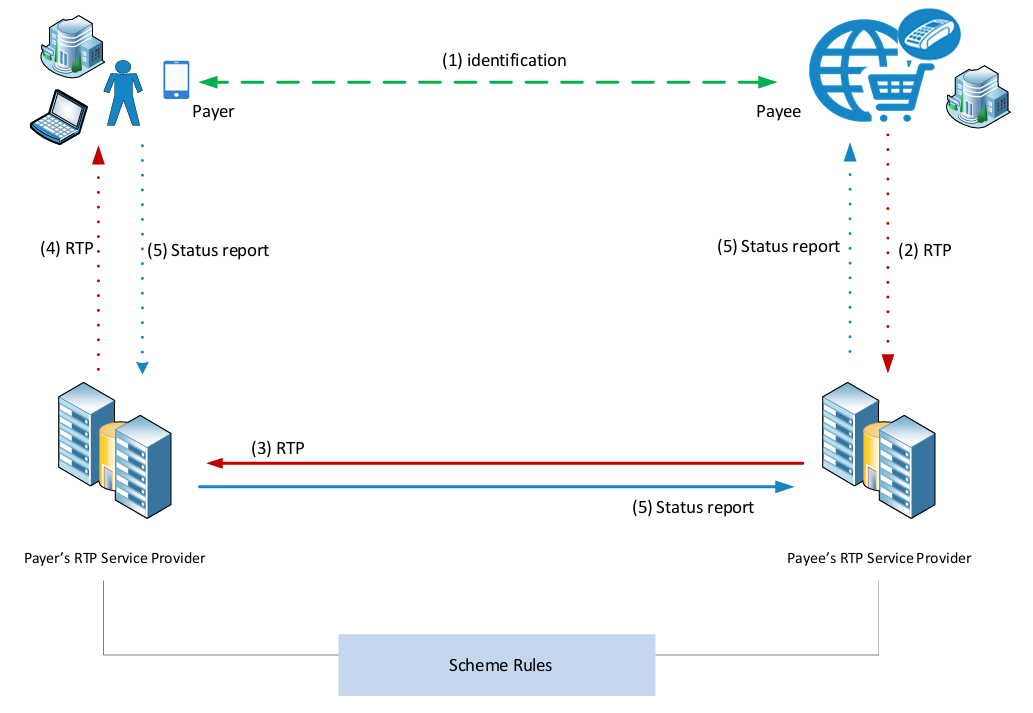
\includegraphics[width=0.8\textwidth]{Imagenes/4CornerModel.png}
  \caption{4CornerModel}
  \label{fig:4corner}
\end{figure}

\begin{table}[htbp]
  \centering
  \caption{Pasos del flujo del esquema SEPA Request-to-Pay (SRTP) y su descripción}
  \label{tab:srtp-steps}
  \begin{tabularx}{\textwidth}{
    @{} 
    >{\raggedright\arraybackslash}p{0.25\textwidth}  % columna fija, alineada a la izquierda
    >{\raggedright\arraybackslash}X                  % columna flexible, alineada a la izquierda
    @{}
  }
    \toprule
    \textbf{Paso} & \textbf{Descripción} \\
    \midrule
    1.\ Identificación
      & Una primera interacción que permite establecer la comunicación entre pagador y beneficiario a través de sus PSP. \\
    2.\ Envío SRTP al PSP del beneficiario
      & El beneficiario envía la SRTP a su propio proveedor de servicios. Este mensaje contiene todos los datos esenciales del esquema RTP. \\
    3.\ Envío SRTP al PSP del pagador
      & El PSP del beneficiario retransmite la SRTP al PSP del pagador. \\
    4.\ Presentación SRTP al pagador
      & La SRTP se muestra al pagador en el canal o dispositivo acordado (aplicación móvil, navegador web, etc.). \\
    5.\ Informe de estado
      & La aceptación o el rechazo de la SRTP por parte del pagador se envía de vuelta al beneficiario a través de sus respectivos PSP. \\
    \bottomrule
  \end{tabularx}
\end{table}

El Operational Scheme Manager (OSM) es la pieza operativa que el EPC ha previsto para ofrecer un servicio centralizado de directorio -el EPC Directory Service (EDS) que facilite la interoperabilidad y el alcance mutuo entre los participantes del esquema SRTP.
La OSM actúa como registro autorizado de todos los PSP y demás actores adheridos al esquema y su misión es garantizas que, en todo momento, cualquier PSP pueda localizar el "endpoint" correcto del PSP objetivo, verificar que está homologado y enviar de forma segura los mensajes SRTP.
Por tanto, para que un PSP pase a formar parte activa del esquema SEPA Request-to-Pay deberá en primer lugar superar con éxito las pruebas de conformidad ISO 20022 y obtener la homologación técnica, tras lo cual acceder al portal de la Operational Scheme Manager para registrar su ficha operativa —incluyendo URL de endpoint, roles SRTP, certificados TLS, claves de firma y datos de contacto 24×7— y aceptar los términos de uso del EPC Directory Service, de modo que la OSM valide la disponibilidad y correcta respuesta de sus endpoints y publique la información correspondiente en el EDS público, quedando accesible al resto de participantes; finalmente, el PSP actualiza sus canales de banca electrónica y/o sus APIs de iniciación de pagos para presentar las solicitudes RTP a sus usuarios, garantizar la autenticación fuerte conforme a PSD2 y gestionar de forma integrada los flujos de aceptación, rechazo y cancelación\paragraph{Flujo básico.}  
El flujo básico de un intercambio RPT es el aiguiente:
\newpage

\begin{figure}[H]
  \centering
  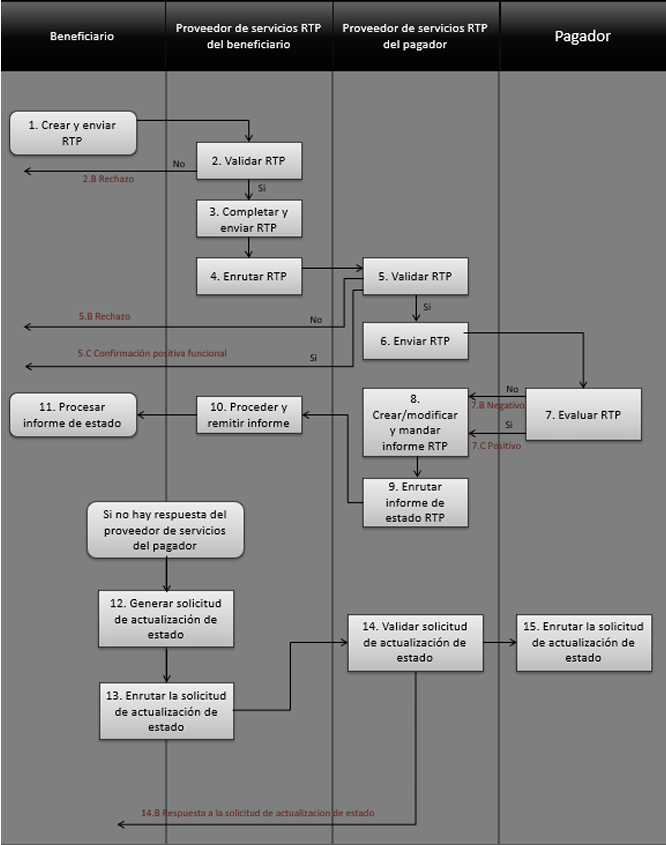
\includegraphics[width=0.95\textwidth, height=0.95\textheight, keepaspectratio]{Imagenes/Flujo.png}
  \label{fig:4corner}
\end{figure}


\setlength{\tabcolsep}{10pt}
\renewcommand{\arraystretch}{1.5}
\begin{longtable}{|p{3cm}|p{12cm}|}
  \hline
  \textbf{Paso/Función} & \textbf{Descripción} \\
  \hline
  \endfirsthead % Encabezado para la primera página

  \hline
  \textbf{Paso/Función} & \textbf{Descripción} \\
  \hline
  \endhead % Encabezado para las páginas siguientes

  \hline
  \multicolumn{2}{|c|}{\textit{(continúa en la siguiente página)}} \\
  \hline
  \endfoot % Pie de página para todas las páginas excepto la última

  \hline
  \multicolumn{2}{|c|}{\textit{Fin de la tabla}} \\
  \hline
  \endlastfoot % Pie de página para la última página

  % Contenido de la tabla
  1 Crear y enviar RTP & El beneficiario crea el "SEPA Request to Pay" SRTP en el formato normalizado (en un formato acordado bilateralmente con su proveedor). Contiene todos los elementos obligatorios y elementos opcionales que puedan ajustarse al flujo en función de las condiciones comerciales. El beneficiario lo envía al proveedor de servicios SRTP del beneficiario. \\
  \hline
  2 Validar RTP & El proveedor de servicios SRTP del beneficiario realiza una primera validación del SRTP. Esto incluye, por ejemplo, validación técnica, de seguridad y de formato (por ejemplo, comprobación del IBAN). \\
  \hline
  2B Rechazo & Si la validación en el paso 2 no tiene éxito, el proveedor de servicios SRTP del beneficiario notifica al beneficiario el rechazo del SRTP, crea un informe de estado negativo y lo envía al beneficiario en el formato acordado con este. \\
  \hline
  3 Completar y enviar RTP & En caso de validación correcta en el paso 2, el proveedor de servicios SRTP del beneficiario enriquece el SRTP con los elementos necesarios para el enrutamiento en el espacio entre proveedores de servicios SRTP y añade un sello de tiempo. \\
  \hline
  4 Enrutar RTP & El SRTP se envía al proveedor de servicios SRTP del pagador en función de los mecanismos de enrutamiento establecidos por el PSP. \\
  \hline
  5 Validar RTP & El proveedor de servicios SRTP del pagador valida el SRTP, incluye la comprobación del identificador del pagador. Esto puede incluir la validación específica del pagador (por ejemplo, si el pagador ha optado por no participar en el servicio, el SRTP es rechazado por defecto). \\
  \hline
  5B Rechazo & Si la validación en el paso 5 no tiene éxito, el proveedor de servicios SRTP del pagador rechaza el SRTP. El proveedor de servicios SRTP del beneficiario y el beneficiario son informados de este rechazo mediante un código de motivo de no aceptación del RTP. \\
  \hline
  5C Confirmación positiva funcional & Después de una validación externa en el paso 5, el proveedor de servicios SRTP confirma al pagador que el proveedor de servicios SRTP ha completado con éxito el procedimiento beneficial. Esta confirmación es obligatoria solo en el caso de que el beneficiario o el proveedor de servicios SRTP no haya confirmado previamente la positividad funcional. \\
  \hline
  6 Enviar RTP & En el caso de validación correcta en el paso 5, el proveedor de servicios SRTP envía el documento SRTP al pagador en el formato acordado (el SRTP puede ser convertido en este paso). \\
  \hline
  7 Evaluar RTP & El pagador decide si aceptar o rechazar el SRTP, determinando el próximo curso de acción. \\
  \hline
  7B Positivo & Si el pagador decide aceptar el SRTP, se envía una respuesta positiva al proveedor de servicios SRTP por parte del pagador. \\
  \hline
  7C Negativo & Si el pagador rechaza el SRTP, se envía una respuesta negativa al proveedor de servicios SRTP por parte del pagador. \\
  \hline
  8 Crear/modificar y mandar informe RTP & El proveedor de servicios SRTP crea un informe informativo basado en la decisión del pagador. Si la decisión es negativa (7B/7C), el informe se envía de vuelta al pagador para su revisión. Si el SRTP ya ha sido aceptado o rechazado, surge un caso excepcional donde no se espera un acuse de recibo. El informe debe considerar la fecha de expiración del SRTP. En este caso, el proveedor de servicios SRTP es responsable de notificar al beneficiario la decisión del proveedor de servicios SRTP, incluyendo el código correspondiente. Como resultado, el beneficiario debe representar el SRTP o utilizar otro canal. \\
  \hline
  9 Enviar informe de estado & El proveedor de servicios SRTP envía un informe de estado actualizado (positivo o negativo) al pagador a través del mismo canal utilizado para el SRTP original, utilizando mecanismos establecidos para la actualización. \\
  \hline
  10 Proceder y remitir informe & El proveedor de servicios SRTP del beneficiario procesa el informe de estado recibido (positivo o negativo), informa al beneficiario y decide los pasos siguientes previo acuerdo con el beneficiario. \\
  \hline
  11 Procesar informe de estado & El beneficiario ejecuta las acciones finales tras la recepción del informe de estado: actualización del estado final del registro SRTP, preparación del pago SRTP conciliación, etc. \\
  \hline
  12 Generar solicitud de actualización de estado & El beneficiario y el proveedor de servicios SRTP del beneficiario pueden enviar una Solicitud de Actualización de Estado si no se ha recibido respuesta hasta la Fecha/Hora de Expiración. \\
  \hline
  13 Enrutar la solicitud de actualización de estado & La solicitud de actualización de estado al proveedor de servicios SRTP del pagador se enruta a través de la misma vía utilizada para el SRTP original basándose en los mecanismos de enrutamiento establecidos. \\
  \hline
  14 Validar solicitud de actualización de estado & Tras la recepción de la solicitud de actualización de estado, el Proveedor de Servicios SRTP del pagador comprueba la validez de la Solicitud. \\
  \hline
  14B Respuesta a la solicitud de actualización de estado & El Proveedor de Servicios SRTP del pagador responde al proveedor de servicios SRTP del beneficiario y, si procede (a través del proveedor de servicios SRTP del beneficiario), al beneficiario (por ejemplo, respuesta del SRTP original no recibida, el pagador aún no ha respondido, etc.). \\
  \hline
  15 Enrutar la solicitud de actualización de estado & En caso de que el pagador aún no haya respondido al SRTP inicial, el proveedor de servicios SRTP del pagador puede enviar la solicitud de actualización de estado al Pagador. \\
  \hline
\end{longtable}

Hay algunos detalles acerca del esquema que conviene aclarar:
\begin{enumerate}
  \item \textbf{Rechazo de un SRTP o una Solicitud de Cancelación (Reject)} \\
        Un "Reject" se produce cuando un SRTP o una Solicitud de Cancelación no es aceptada antes de ser enviada al siguiente participante en la cadena de pago. El mensaje de rechazo sigue la misma ruta que el SRTP original sin modificar ningún dato, y se incluye un registro con los detalles necesarios para asegurar un rastro de auditoría. Además, el mensaje de rechazo lleva un código de motivo que explica la razón del rechazo. La identificación del SRTP original se hace mediante la referencia única incluida por el proveedor de servicios del receptor. Los rechazos se envían de manera instantánea por el proveedor de servicios SRTP que no puede procesar la solicitud, y estos rechazos pueden ser generados automáticamente en función de comprobaciones técnicas o comerciales, sin intervención del pagador.

  \item \textbf{Respuestas a un SRTP (positiva o negativa)} \\
        Cuando un pagador responde a un SRTP, puede aceptar (respuesta positiva) o rechazarlo (respuesta negativa). En ambos casos, el mensaje sigue la misma ruta que el SRTP original, sin alterar los datos, y se envía instantáneamente entre los proveedores de servicios SRTP. Las respuestas negativas incluyen un código de motivo que especifica la razón del rechazo, mientras que las respuestas positivas simplemente confirman la aceptación de la solicitud. Como en el caso de los rechazos, se mantiene un registro detallado de los datos relevantes para asegurar la trazabilidad del proceso y la transparencia en la comunicación entre los proveedores de servicios.

  \item \textbf{Solicitud de Cancelación del SRTP} \\
        Una “Request for cancelation” RfC puede ser iniciada por el y se transmite al pagador a través de los proveedores de servicios SRTP. La solicitud sigue la misma ruta que el SRTP original, sin modificar los datos, y debe incluir un código de motivo (atributo AT-R106) que justifique la cancelación. Esta solicitud puede realizarse hasta la fecha de expiración del SRTP, a menos que ya haya sido rechazado, cancelado o expirado. El proveedor de servicios SRTP del pagador verifica la validez de la solicitud antes de reenviarla, y si no se puede procesar, envía una respuesta negativa. Si la cancelación se ejecuta correctamente, el proveedor del pagador envía una respuesta positiva de manera instantánea, manteniendo siempre un registro para garantizar la trazabilidad del proceso.
\end{enumerate}
%%%%%%%%%%%%%%%%%%%%%%%%%%%%%%%%%%%%%%%%%%%%%%%%%%%%%%%%%%%%%%%%%%%%%%%%%%%%%%%%%%%%%%%%%%%%%%%%%%%%%%%%%%%%%%%%%%
%%%%%%%%%%%%%%%%%%%%%%%%%%%%%%%%%%%%%%%%%%%%%%%%%%%%%%%%%%%%%%%%%%%%%%%%%%%%%%%%%%%%%%%%%%%%%%%%%%%%%%%%%%%%%%%%%%
\paragraph{Casos de uso representativos.}
El \textbf{SEPA Request-to-Pay} se concibió como un servicio versátil, capaz de cubrir desde pagos cotidianos de bajo valor hasta cobros empresariales complejos. No obstante, el caso de uso considerado más transformador—y sobre el que se centra este TFG—es la \emph{sustitución del adeudo directo SEPA (SDD) en pagos recurrentes}. Aun así, existen otros escenarios relevantes que merece la pena describir para contextualizar el alcance potencial de SRTP.

\begin{enumerate}
    \item \textbf{Punto de Venta Físico (POS)}
    \begin{itemize}
        \item \textbf{Descripción:} Este caso de uso de Request to Pay se emplea en tiendas físicas, donde el payee (el comercio) envía una solicitud de pago al payor (el cliente) utilizando un código QR o una tecnología NFC (Near Field Communication). Al escanear el código QR con su móvil o usar NFC en la terminal de pago, el cliente es redirigido a su aplicación bancaria para autorizar el pago de manera inmediata.
        \item \textbf{Proceso de Identificación:}
        \begin{itemize}
            \item \textit{Identificación del Payor:} El payor se autentica directamente en su aplicación bancaria, generalmente mediante su número de cuenta bancaria, número de tarjeta, o métodos de autenticación biométrica o PIN, según lo permita la aplicación del banco.
            \item \textit{Identificación del Payee:} El payee está identificado en el sistema mediante un ID de comercio asociado a la terminal de pago o al código QR/NFC escaneado por el cliente. Estos elementos proporcionan los datos necesarios para vincular la solicitud de pago al comercio correspondiente.
        \end{itemize}
        \item \textbf{Proceso de Pago:}
        \begin{itemize}
            \item El cliente escanea el código QR o se conecta mediante NFC a la terminal de pago.
            \item La aplicación bancaria del cliente recibe la solicitud de pago con el monto y la referencia.
            \item El cliente revisa la información y autoriza el pago, un proceso rápido y conveniente, crucial en entornos físicos donde la velocidad es esencial.
        \end{itemize}
        \item \textbf{Diferencias Clave:}
        \begin{itemize}
            \item La rapidez y conveniencia son fundamentales en este caso de uso. El proceso de identificación y autorización es sencillo y rápido, requiriendo solo la confirmación del cliente a través de su banco, típicamente con autenticación biométrica o PIN.
            \item Es ideal para transacciones de bajo valor donde la experiencia del cliente es un factor determinante.
        \end{itemize}
    \end{itemize}

    \item \textbf{Comercio Electrónico (E-commerce)}
    \begin{itemize}
        \item \textbf{Descripción:} En este caso, el payee (el comercio electrónico) envía una solicitud de pago al payor (el cliente) durante el proceso de checkout o mediante un enlace de pago enviado a través de una aplicación bancaria o correo electrónico. El cliente es redirigido a su aplicación bancaria, donde debe autenticarse y revisar los detalles antes de aprobar el pago.
        \item \textbf{Proceso de Identificación:}
        \begin{itemize}
            \item \textit{Identificación del Payor:} La identificación implica un proceso de autenticación multifactor (por ejemplo, contraseña, token de seguridad o autenticación biométrica) para garantizar la seguridad de la transacción, realizado en la aplicación bancaria o la página de pago del comercio.
            \item \textit{Identificación del Payee:} El payee se identifica mediante un ID de comercio electrónico que incluye su nombre comercial, identificador fiscal, número de cuenta o un identificador único en la plataforma de pagos.
        \end{itemize}
        \item \textbf{Proceso de Pago:}
        \begin{itemize}
            \item El cliente recibe la solicitud de pago a través de un enlace en el checkout o en su aplicación bancaria.
            \item El cliente se autentica en su aplicación bancaria, revisa el monto, la referencia y los detalles del comerciante, y aprueba el pago.
            \item Una vez validada, el dinero se transfiere de manera segura.
        \end{itemize}
        \item \textbf{Diferencias Clave:}
        \begin{itemize}
            \item A diferencia del punto de venta físico, el proceso en comercio electrónico es más lento debido a la autenticación adicional y la revisión en línea.
            \item La seguridad es prioritaria, dado el mayor riesgo de fraude en transacciones digitales.
        \end{itemize}
    \end{itemize}

    \item \textbf{Facturación Electrónica (E-invoicing)}
    \begin{itemize}
        \item \textbf{Descripción:} Común en empresas que envían facturas electrónicas, el payee (la empresa emisora) envía una solicitud de pago con los detalles de la factura al payor (el cliente). El cliente recibe la solicitud en su correo electrónico o aplicación bancaria, pudiendo revisar los detalles antes de decidir cuándo pagar.
        \item \textbf{Proceso de Identificación:}
        \begin{itemize}
            \item \textit{Identificación del Payor:} El payor se identifica mediante su número de cliente, correo electrónico o número de cuenta bancaria vinculado a la empresa emisora.
            \item \textit{Identificación del Payee:} El payee se identifica por su NIF (Número de Identificación Fiscal) o un ID de facturación electrónica único, asegurando la verificación de la entidad receptora.
        \end{itemize}
        \item \textbf{Proceso de Pago:}
        \begin{itemize}
            \item El cliente recibe la factura y la solicitud de pago por correo o notificación bancaria.
            \item Tras validar la información, autoriza el pago a través de su aplicación bancaria, completando la transacción.
        \end{itemize}
        \item \textbf{Diferencias Clave:}
        \begin{itemize}
            \item Ofrece flexibilidad, permitiendo al cliente revisar la factura antes de pagar.
            \item La identificación del payee incluye detalles fiscales, incrementando la seguridad en la validación.
        \end{itemize}
    \end{itemize}

    \item \textbf{Pagos Recurrentes}
    \begin{itemize}
        \item \textbf{Descripción:} Ideal para suscripciones o pagos periódicos (streaming, software en la nube, gimnasios), el payor autoriza la primera transacción para suscribirse. Los pagos posteriores se gestionan automáticamente según la periodicidad acordada, sin intervención adicional.
        \item \textbf{Proceso de Identificación:}
        \begin{itemize}
            \item \textit{Identificación del Payor:} El payor autoriza la primera transacción con autenticación en su aplicación bancaria (cuenta, contraseña o biométrica).
            \item \textit{Identificación del Payee:} El payee se identifica por su ID de suscripción y número de cuenta para configurar los pagos recurrentes.
        \end{itemize}
        \item \textbf{Proceso de Pago:}
        \begin{itemize}
            \item El cliente autoriza el pago inicial.
            \item Los cobros posteriores se realizan automáticamente según la periodicidad (mensual, anual, etc.).
        \end{itemize}
        \item \textbf{Diferencias Clave:}
        \begin{itemize}
            \item Se distingue por la automatización tras la autorización inicial, reduciendo la intervención del cliente.
            \item La comodidad y la automatización son sus principales ventajas.
        \end{itemize}
    \end{itemize}

    \item \textbf{Pagos de Grandes Montos}
    \begin{itemize}
        \item \textbf{Descripción:} Utilizado en transacciones de alto valor (compras importantes, bienes de gran valor), este caso requiere métodos adicionales de autenticación para garantizar la seguridad.
        \item \textbf{Proceso de Identificación:}
        \begin{itemize}
            \item \textit{Identificación del Payor:} El payor usa autenticación robusta (OTP, tokens de seguridad o multifactor como PIN y biométrica) para validar la transacción.
            \item \textit{Identificación del Payee:} El payee es una entidad registrada con un identificador único (ID de comerciante), asegurando el destinatario correcto.
        \end{itemize}
        \item \textbf{Proceso de Pago:}
        \begin{itemize}
            \item El payor revisa el monto y autoriza el pago con autenticación adicional.
            \item Tras verificar la identidad, el pago se completa.
        \end{itemize}
        \item \textbf{Diferencias Clave:}
        \begin{itemize}
            \item Requiere autenticación más fuerte debido al alto riesgo de fraude en grandes sumas.
            \item La seguridad es el factor más crítico, priorizando la protección contra fraudes y errores.
        \end{itemize}
    \end{itemize}
\end{enumerate}
%%%%%%%%%%%%%%%%%%%%%%%%%%%%%%%%%%%%%%%%%%%%%%%%%%%%%%%%%%%%%%%%%%%%%%%%%%%%%%%%%%%%%%%%%%%%%%%%%%%%%%%%%%%%%%%%%%
%%%%%%%%%%%%%%%%%%%%%%%%%%%%%%%%%%%%%%%%%%%%%%%%%%%%%%%%%%%%%%%%%%%%%%%%%%%%%%%%%%%%%%%%%%%%%%%%%%%%%%%%%%%%%%%%%%
\subsection{RTP dentro del ecosistema de pagos: arquitectura en capas}
\label{subsec:cubo-pagos}

El ecosistema de pagos SEPA (Zona Única de Pagos en Euros) se puede describir mediante capas jerárquicas, desde los usuarios finales hasta las infraestructuras financieras que ejecutan las transacciones. A continuación se detallan las principales capas del modelo actual de pagos SEPA:

\begin{description}
  \item[\textbf{Capa de usuarios finales}] 
    En la capa más alta se encuentran el \emph{pagador} (ordenante del pago) y el \emph{beneficiario} (cobrador). Son quienes inician y reciben los pagos, respectivamente, ya sea personas o empresas involucradas en una transacción.

  \item[\textbf{Capa de iniciación o interacción}] 
    Es donde se produce la solicitud o autorización del pago a través de algún canal o interfaz. Por ejemplo, en pagos SEPA tradicionales el pagador suele autorizar una transferencia mediante la banca online o una aplicación móvil. En entornos de comercio electrónico o físico, esta capa correspondería al proceso de \emph{checkout} (por ejemplo, introduciendo datos en una pasarela de pago online o mediante un TPV/POS en tienda).

  \item[\textbf{Capa de proveedores de servicios de pago (PSP)}] 
    Aquí actúan las entidades financieras o PSP de cada parte. Típicamente, el banco del pagador y el banco del beneficiario son quienes ofrecen las cuentas bancarias y servicios de pago a sus clientes. Estas entidades facilitan la emisión y recepción de órdenes de pago en nombre de los usuarios finales.

  \item[\textbf{Capa de esquemas de pago}] 
    Es el conjunto de reglas y estándares comunes que permiten la interoperabilidad entre todos los PSP. En SEPA, por ejemplo, existen los esquemas de transferencia crediticia (SCT, SCT Inst) y adeudo directo (SDD), definidos por el European Payments Council (EPC). Cada esquema asegura que, independientemente del banco involucrado, un pago en euros siga las mismas normas y formatos. Un esquema de pago no es el movimiento del dinero en sí, sino el conjunto de reglas, mensajes e infraestructura técnica que orquesta cómo se inician y gestionan esos pagos.

  \item[\textbf{Capa de infraestructuras de compensación}] 
    Son las plataformas interbancarias que procesan las transacciones según las reglas del esquema. En SEPA, existen cámaras de compensación automatizadas (CSM) y redes de pago instantáneo. Por ejemplo, el sistema STEP2 de EBA Clearing procesa transferencias SEPA diarias, mientras que para pagos instantáneos existen redes 24/7 como TIPS (del BCE) o RT1 (de EBA Clearing). Estas infraestructuras se encargan de intercambiar las órdenes de pago entre el banco emisor y el banco receptor, aplicando compensación multilateral si procede.

  \item[\textbf{Capa de liquidación}] 
    Es la capa más baja, donde se realiza la liquidación final de fondos entre bancos. Normalmente ocurre en los bancos centrales u organismos de compensación: por ejemplo, las obligaciones netas resultantes de muchas transacciones SEPA pueden liquidarse en TARGET2 (sistema del Banco Central Europeo). En pagos inmediatos, la liquidación suele ser casi en tiempo real (por ejemplo, mediante TIPS que liquida cada operación al momento en cuentas del banco central).
\end{description}

\begin{figure}[H]
  \centering
  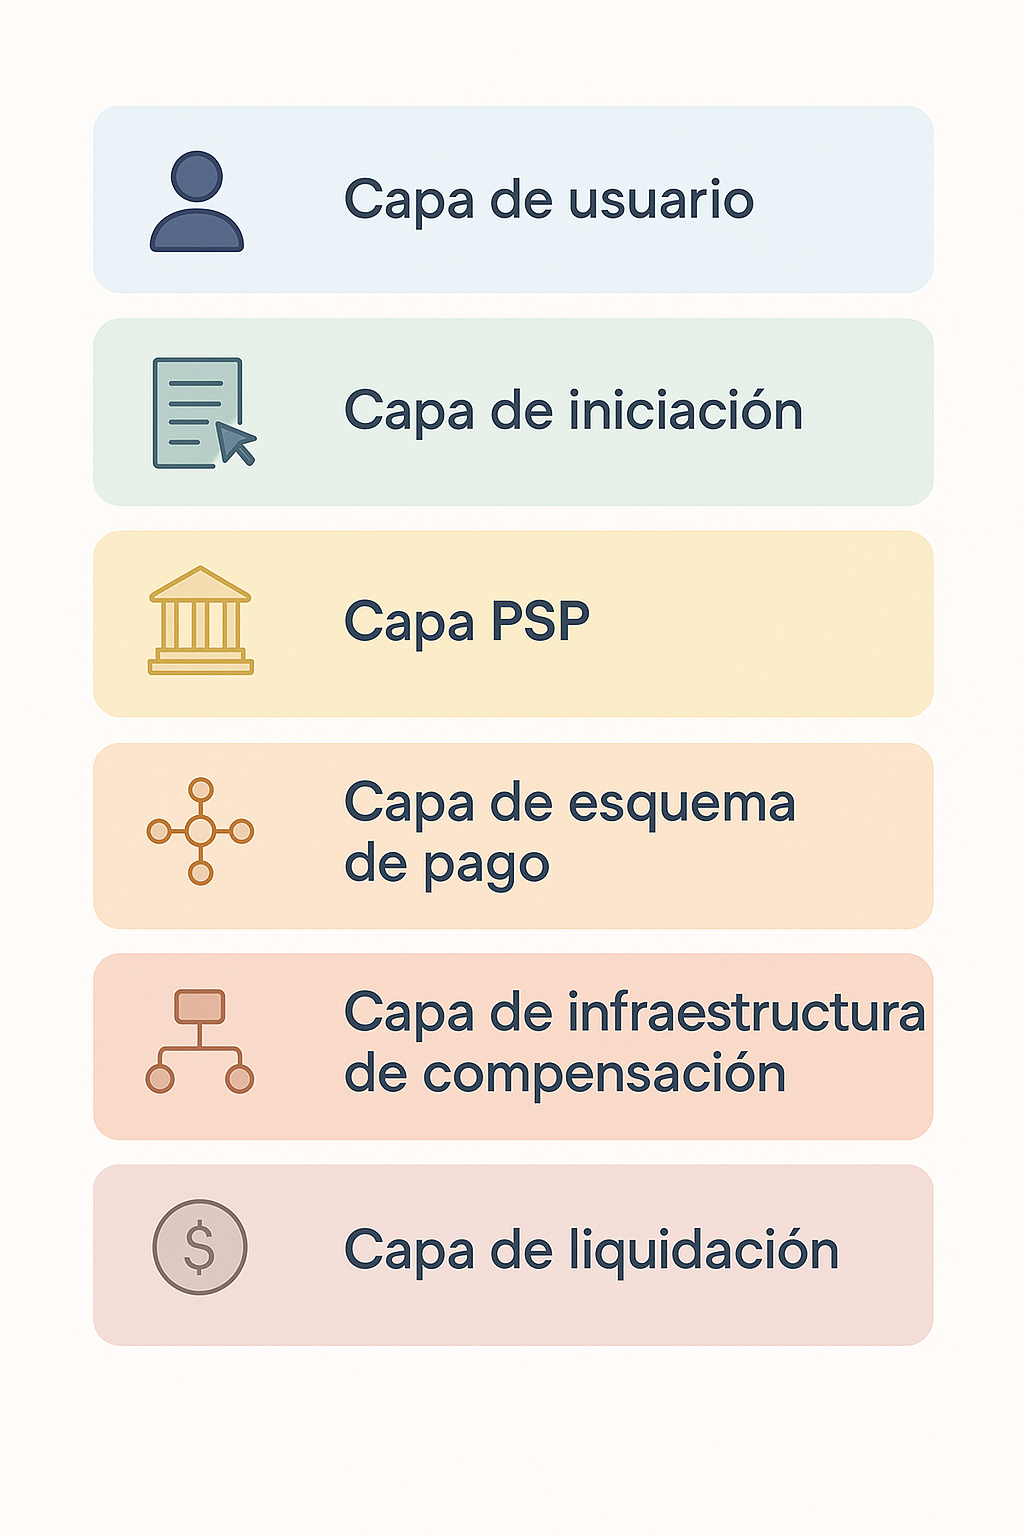
\includegraphics[width=0.5\textwidth]{Imagenes/esq1.png}
  \caption{Layer}
  \label{fig:4corner}
\end{figure}

Esta arquitectura por capas garantiza que un pago iniciado por un usuario en un banco pueda llegar a otro usuario en distinto banco de forma segura, eficiente e interoperable en toda la zona euro. Cada capa agrega funciones específicas: los usuarios generan órdenes, los PSP las gestionan, los esquemas proporcionan las reglas comunes, y las infraestructuras las ejecutan y asientan los fondos en última instancia.

RTP es un nuevo servicio/esquema incorporado en la arquitectura SEPA que se sitúa principalmente en la capa de esquema de pago, actuando como una capa adicional de mensajería sobre los instrumentos de pago existentes.

%----------------------------------------------------------------------
\subsubsection*{Ejemplo comparado: pago con tarjeta vs.\ RTP}

Como muestra el esquema comparativo, los pagos con tarjeta (ej.\ Visa/Mastercard) históricamente han operado con una arquitectura de funciones similar a la de SEPA, pero con diferencias en los actores y procesos de cada capa:

\begin{description}
  \item[\textbf{Usuarios (pagador/beneficiario)}]
    En tarjetas, el pagador es el \emph{titular de la tarjeta} y el beneficiario es el \emph{comercio} que recibe el pago. En esencia es equivalente al ordenante y beneficiario de una transferencia, con la diferencia de que el pagador utiliza un instrumento distinto (su tarjeta en lugar de una cuenta bancaria directa).

  \item[\textbf{PSP / entidades}]
    En el modelo de cuatro partes de las tarjetas interviene el \emph{banco emisor} (emite la tarjeta al pagador) y el \emph{banco adquirente} (procesa pagos para el comerciante). Estos roles son análogos a la entidad del pagador y del beneficiario en SEPA, pero en el mundo tarjeta suelen implicar acuerdos específicos (p.\,ej.\,el comerciante contrata un adquirente para aceptar Visa/Mastercard). En cambio, en SEPA cualquier banco puede enviar o recibir transferencias para un cliente sin acuerdos individuales con cada comercio, ya que todos siguen el esquema común.

  \item[\textbf{Esquema de pago}]
    Las tarjetas operan bajo esquemas propietarios como Visa, Mastercard, etc., que definen reglas, formatos de mensajes (p.\,ej.\ mensajes de autorización y liquidación) y que actúan también como redes de procesamiento. Son equivalentes a los esquemas SEPA en cuanto a que proveen interoperabilidad, pero controlados por empresas particulares. El esquema Visa/Mastercard indica cómo se autoriza una compra, cómo se liquida posteriormente y fija también aspectos comerciales como las tasas de intercambio entre emisor y adquirente. En SEPA, el esquema SRTP + SCT Inst provee una funcionalidad comparable de solicitud y pago, pero dentro de un marco colaborativo paneuropeo. De hecho, SRTP adopta un modelo muy similar al de tarjetas de cuatro partes (pagador, beneficiario y sus respectivos proveedores), tanto que el EPC prevé que incluso podrían llegar a existir comisiones de intercambio análogas en este ecosistema\footnote{\url{https://redbridgedta.com}} (aunque inicialmente SRTP nace sin tarifas de intercambio explícitas).

  \item[\textbf{Infraestructura de compensación}]
    En los pagos con tarjeta, la red del esquema (p.\,ej.\ VisaNet) se encarga de la autorización instantánea de la transacción y de la compensación/clearing de las transacciones entre emisores y adquirentes. Visa o Mastercard centralizan el intercambio de mensajes financieros. En SEPA, por el contrario, las compensaciones suelen realizarse a través de múltiples infraestructuras (por ejemplo, cámaras como STEP2 o servicios inmediatos como TIPS) que no pertenecen a una sola empresa sino que son parte del ecosistema colaborativo europeo. Con Request to Pay, la mensajería de solicitud viaja por la red designada (p.\,ej.\ la plataforma R2P de EBA Clearing) y el pago resultante se compensa a través de los \emph{rails} SEPA existentes (p.\,ej.\ RT1/TIPS para instantáneas).

  \item[\textbf{Liquidación final}]
    En ambos casos, finalmente hay un traspaso de fondos entre bancos. En las tarjetas, las marcas de tarjeta calculan las obligaciones netas entre cada banco emisor y adquirente y típicamente las liquidan al final del día a través de cuentas en un banco central u otros mecanismos interbancarios. En SEPA, cada transferencia individual (especialmente si es instantánea) puede liquidarse inmediatamente en el banco central. Desde el punto de vista de capas, ambos mundos terminan convergiendo en la necesidad de que el dinero se ajuste entre las cuentas de los bancos participantes.
\end{description}

\begin{figure}[H]
  \centering
  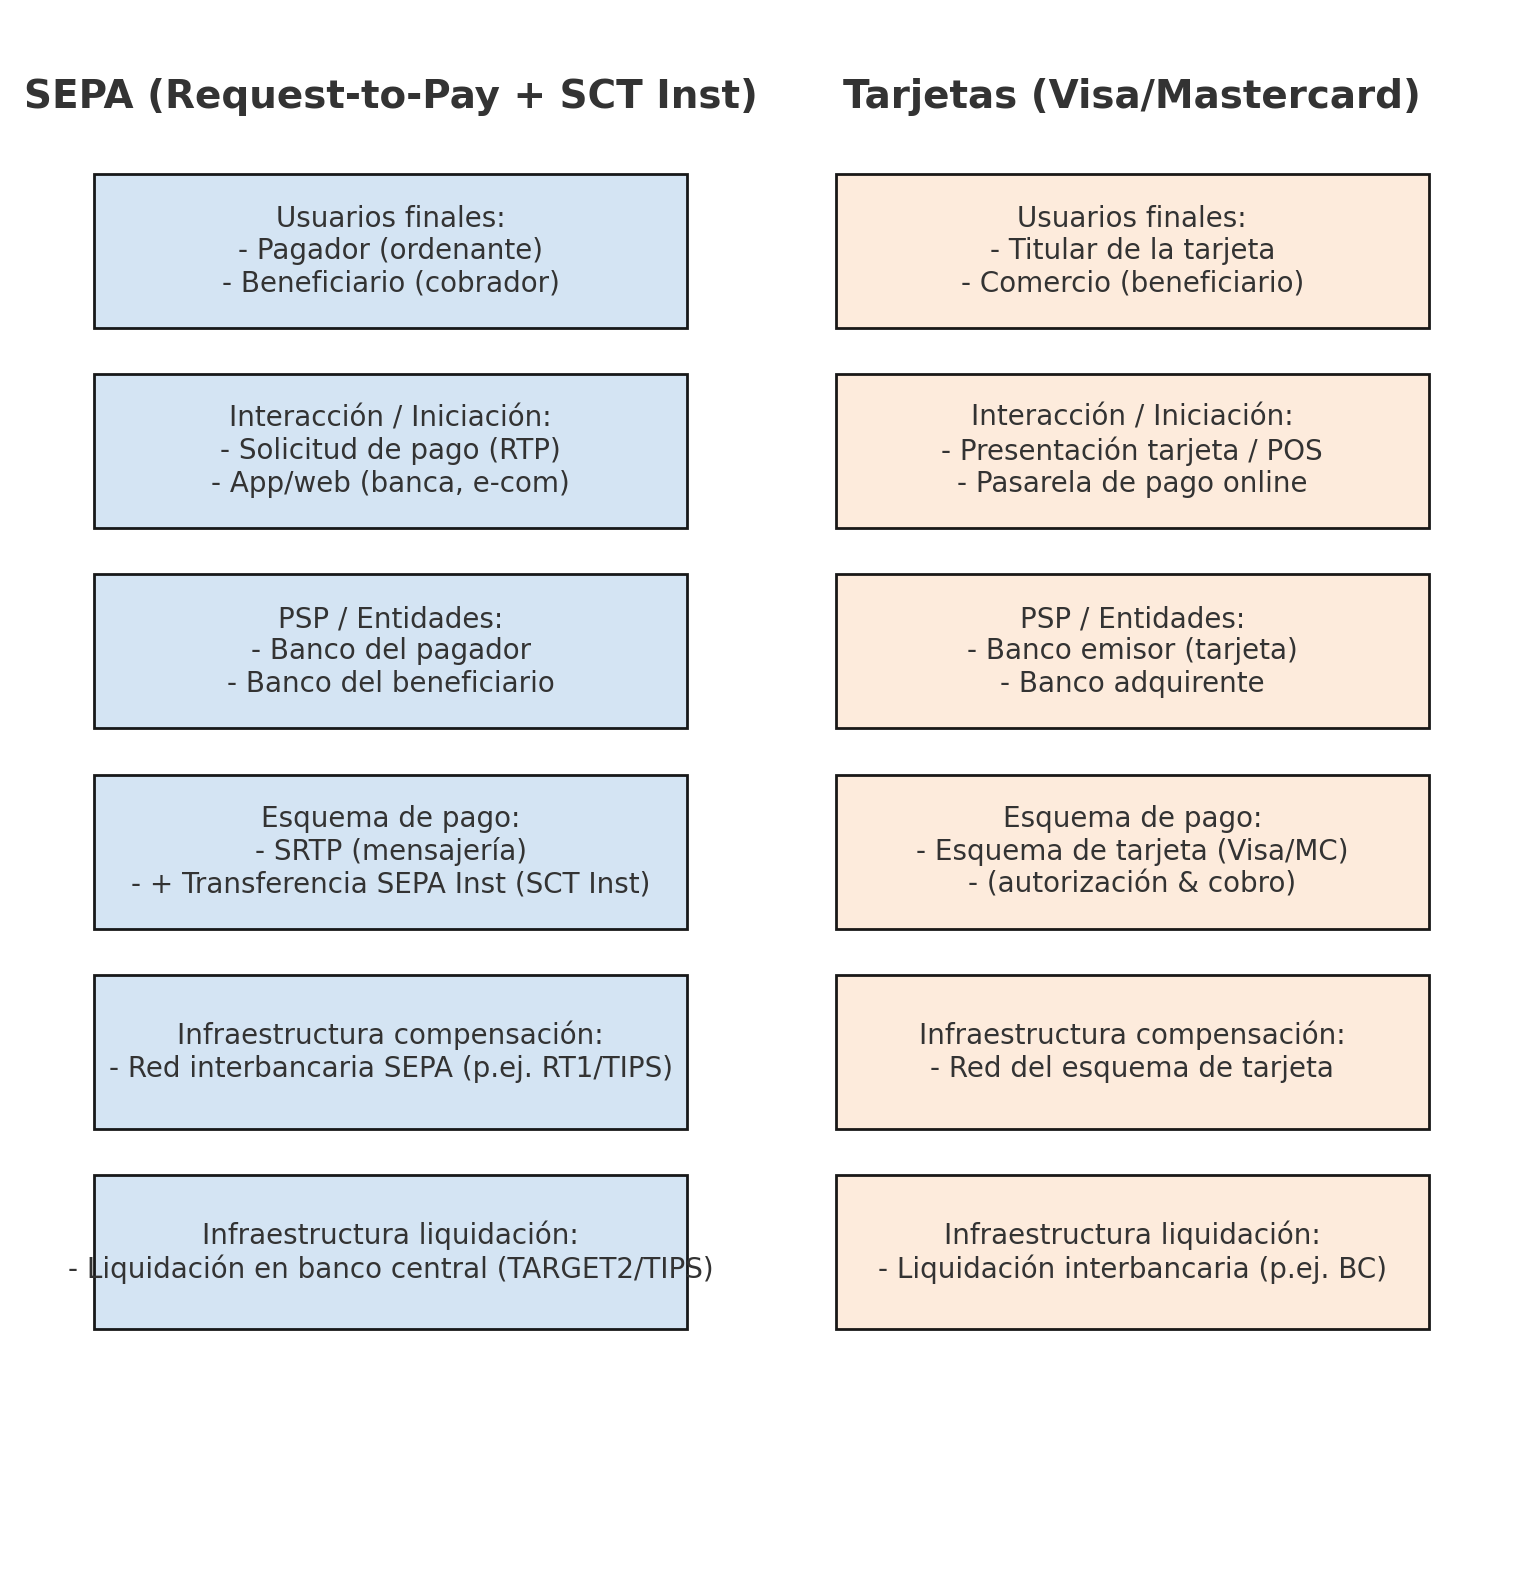
\includegraphics[width=0.8\textwidth]{Imagenes/LayerComp.png}
  \caption{LayerComp}
  \label{fig:4corner}
\end{figure}

\bigskip

\noindent\textbf{¿Qué simplifica o elimina Request to Pay respecto al modelo de tarjetas?}

Principalmente, elimina intermediarios dedicados y procesos redundantes. Por ejemplo, en un pago SRTP + SCT Inst no es necesario un procesador/acquirente específico ni una red de tarjetas propietaria, ya que los propios bancos de pagador y beneficiario se comunican directamente mediante el esquema común\footnote{\url{https://cpg.de}, \url{https://redbridgedta.com}}. Esto puede reducir costes de aceptación para el comercio (evitando comisiones elevadas de tarjetas) y simplifica la integración: el comercio recibe el dinero directamente en su cuenta bancaria vía SEPA, sin pasos intermedios de recibir fondos a través de entidades de tarjeta y luego liquidarlos. Además, no se requiere que el pagador proporcione datos sensibles como el PAN de tarjeta o incluso su IBAN al comercio; la solicitud llega por canales bancarios seguros y el cliente simplemente autoriza en su entorno bancario\footnote{\url{https://docs.monei.com}}. En resumen, Request to Pay se apoya en la infraestructura bancaria existente (cuentas y pagos inmediatos) para ofrecer una experiencia similar a la de tarjeta, pero con menos capas propietarias, aprovechando la red SEPA ya desplegada en toda Europa.


%----------------------------------------------------------------------
% FIN DE BLOQUE
%----------------------------------------------------------------------

